\documentclass{article}
\usepackage[paperwidth=6.1in,paperheight=3.1in,margin=0in]{geometry}
\usepackage{mathptmx}%{times}
\usepackage{graphicx}
\usepackage{siunitx}
\usepackage[absolute,overlay]{textpos}
\usepackage{color}
\usepackage{tikz}
\usetikzlibrary{decorations.markings}
\tikzset{>=latex}

\setlength{\parindent}{0pt}
\definecolor{gnuplotred}{HTML}{e51e10}
\begin{document}
\TPMargin{2pt}
\centering
\includegraphics{../mountainAdvection-btf-5000-linearUpwind-1000/constant/meshW.pdf} \\
\includegraphics{../mountainAdvection-cutCell-5000-linearUpwind-1000/constant/meshW.pdf} \\
\hspace*{0.8em}\includegraphics{../mountainAdvection-slantedCell-5000-linearUpwind-1000/constant/mesh.pdf}

% (a) streamlines
\begin{textblock}{5}(1.84,0.78)
\textblockcolour{}
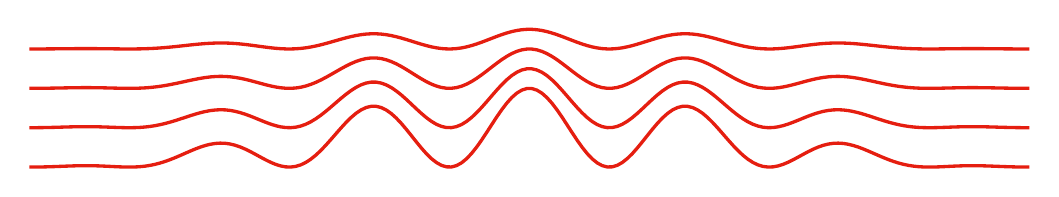
\begin{tikzpicture}[xscale=0.254,yscale=0.2]
	\draw [line width=1.2pt,color=gnuplotred,domain=-25:25,samples=200] plot (\x,{5*cos(deg(\x*3.14159/8))*cos(deg(\x*3.14159/8))*cos(deg(\x*3.14159/50))*cos(deg(\x*3.14159/50))});

	\draw [line width=1.2pt,color=gnuplotred,domain=-25:25,samples=200] plot (\x,{2.5 + (1 - 2.5/10)*5*cos(deg(\x*3.14159/8))*cos(deg(\x*3.14159/8))*cos(deg(\x*3.14159/50))*cos(deg(\x*3.14159/50))});
	
	\draw [line width=1.2pt,color=gnuplotred,domain=-25:25,samples=200] plot (\x,{5 + (1 - 5/10)*5*cos(deg(\x*3.14159/8))*cos(deg(\x*3.14159/8))*cos(deg(\x*3.14159/50))*cos(deg(\x*3.14159/50))});

	\draw [line width=1.2pt,color=gnuplotred,domain=-25:25,samples=200] plot (\x,{7.5 + (1 - 7.5/10)*5*cos(deg(\x*3.14159/8))*cos(deg(\x*3.14159/8))*cos(deg(\x*3.14159/50))*cos(deg(\x*3.14159/50))});
\end{tikzpicture}
\end{textblock}

% (b) streamlines
\begin{textblock}{5}(1.84,5.78)
\textblockcolour{}
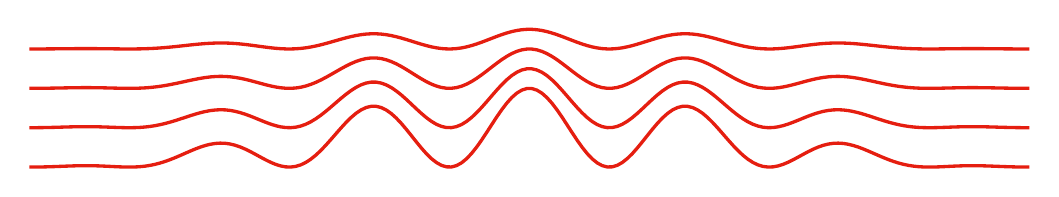
\begin{tikzpicture}[xscale=0.254,yscale=0.2]
	\draw [line width=1.2pt,color=gnuplotred,domain=-25:25,samples=200,postaction={decorate}] plot (\x,{5*cos(deg(\x*3.14159/8))*cos(deg(\x*3.14159/8))*cos(deg(\x*3.14159/50))*cos(deg(\x*3.14159/50))});

	\draw [line width=1.2pt,color=gnuplotred,domain=-25:25,samples=200] plot (\x,{2.5 + (1 - 2.5/10)*5*cos(deg(\x*3.14159/8))*cos(deg(\x*3.14159/8))*cos(deg(\x*3.14159/50))*cos(deg(\x*3.14159/50))});
	
	\draw [line width=1.2pt,color=gnuplotred,domain=-25:25,samples=200] plot (\x,{5 + (1 - 5/10)*5*cos(deg(\x*3.14159/8))*cos(deg(\x*3.14159/8))*cos(deg(\x*3.14159/50))*cos(deg(\x*3.14159/50))});

	\draw [line width=1.2pt,color=gnuplotred,domain=-25:25,samples=200] plot (\x,{7.5 + (1 - 7.5/10)*5*cos(deg(\x*3.14159/8))*cos(deg(\x*3.14159/8))*cos(deg(\x*3.14159/50))*cos(deg(\x*3.14159/50))});
\end{tikzpicture}
\end{textblock}

% (c) streamlines
\begin{textblock}{5}(1.84,10.81)
\textblockcolour{}
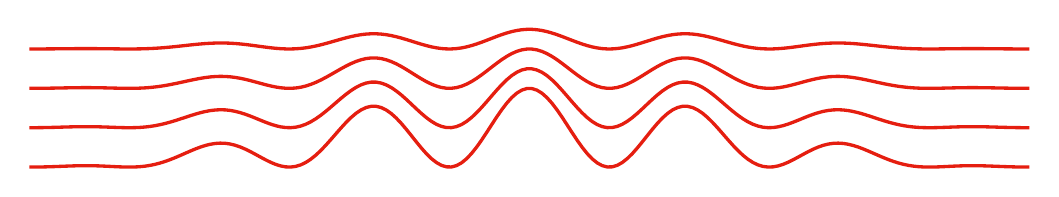
\begin{tikzpicture}[xscale=0.254,yscale=0.2]
	\draw [line width=1.2pt,color=gnuplotred,domain=-25:25,samples=200] plot (\x,{5*cos(deg(\x*3.14159/8))*cos(deg(\x*3.14159/8))*cos(deg(\x*3.14159/50))*cos(deg(\x*3.14159/50))});

	\draw [line width=1.2pt,color=gnuplotred,domain=-25:25,samples=200] plot (\x,{2.5 + (1 - 2.5/10)*5*cos(deg(\x*3.14159/8))*cos(deg(\x*3.14159/8))*cos(deg(\x*3.14159/50))*cos(deg(\x*3.14159/50))});
	
	\draw [line width=1.2pt,color=gnuplotred,domain=-25:25,samples=200] plot (\x,{5 + (1 - 5/10)*5*cos(deg(\x*3.14159/8))*cos(deg(\x*3.14159/8))*cos(deg(\x*3.14159/50))*cos(deg(\x*3.14159/50))});

	\draw [line width=1.2pt,color=gnuplotred,domain=-25:25,samples=200] plot (\x,{7.5 + (1 - 7.5/10)*5*cos(deg(\x*3.14159/8))*cos(deg(\x*3.14159/8))*cos(deg(\x*3.14159/50))*cos(deg(\x*3.14159/50))});
\end{tikzpicture}
\end{textblock}
\begin{textblock}{4}(2,0.5)
\normalsize
\textblockcolour{white}
(a) Basic terrain-following
\end{textblock}
\begin{textblock}{2}(2,5.5)
\normalsize
\textblockcolour{white}
(b) Cut cells
\end{textblock}
\begin{textblock}{2.5}(2,10.5)
\normalsize
\textblockcolour{white}
(c) Slanted cells
\end{textblock}
\end{document}
